%%%%%%%%%%%%%%%%%%%% author.tex %%%%%%%%%%%%%%%%%%%%%%%%%%%%%%%%%%%
%
% sample root file for your "contribution" to a proceedings volume
%
% Use this file as a template for your own input.
%
%%%%%%%%%%%%%%%% Springer %%%%%%%%%%%%%%%%%%%%%%%%%%%%%%%%%%


\documentclass[12pt]{svproc}
\usepackage{graphicx}
\graphicspath{ {/figures/} }
\usepackage{url}
\usepackage[export]{adjustbox}
\usepackage{subcaption}
\captionsetup{compatibility=false}
\usepackage[utf8]{inputenc}
\usepackage{wrapfig}
\usepackage{amsmath}
\usepackage{amssymb}
\usepackage{minted}
\usepackage{inputenc}


\usepackage[left=1in,right=1in,top=1in,bottom=1in,footskip=0.25in]{geometry}


\def\UrlFont{\rmfamily}

\begin{document}
	


\title{Application of Greedy Algorithm for Unmixing of Hyperspectral data}

%
\author{}
\institute{By Vanshika Gupta(16CV245)\\Mini Project(AM380) Report\\National Institute of Technology Karnataka, Surathkal\\~\\ 
Guided by Ms.Amba Shetty \\
Department of Applied Mechanics and Hydraulics\\
National Institute of Technology Karnataka, Surathkal\\
}


\maketitle              % typeset the title of the contribution
%

\section{\Large Abstract}
Our objective for this course is to study Hyperspectral Unmixing and the different approaches that have been developed to solve this problem statemnt. In this course, we  study about what is hyperspectral unmixing, its importance in real world applications and algorithms developed. We will be working on one processing technique to obtain the amount of noise in the image ie. the Signal-to-noise spectral distibution(SNR-SD) for usage of hyperspectral data. Also, we have looked into an algorithm proposed recently to solve the unmixing problem known as the Greedy Algorithm or the Greedy Sparse approximation. We will look into its code implimentation on a synthetically created image and further look into its application on real world data. 


\section[60pt]{\Large Introduction}
%
Hyperspectral remote sensing, also sometimes called Imaging Spectroscopy, is used to capture data in hundreds of contiguous narrow bands of the electromagnetic spectrum. It allows whole spectral curves to be recorded with individual absorption features, therefore, providing information related to surface material that can be exploited to characterize, quantify and perform automated detection of the targets of interest with much better accuracy than multispectral or RGB image. \\

Modern spaceborne and airborne hyperspectral sensors measure the reflectance of the Earth's surface at hundreds of contiguous narrow bands, which results in hyperspectral image cubes with two spatial and one spectral dimension. Each pixel of a hyperspectal image is a vector that represents a spectral signature measured by the sensor. Due to low spatial resolution of the sensors and multiple scatterings, the spectra at a pixel is usually a mixture of multiple pure spectra or endmemembers, corresponding to different materials on the ground. Hyperspectral unmixing aims at identifying the endmembers in a mixed pixel and computing their fractional abundances i.e. their proportion in the pixel. Unmxing of the hyperspectral images is considered a major challenge in remote sensing data analysis.\\

In hyperspectral imagery, one pixel typically consists of a mixture of the reflectance spectra of several materials, where the mixture coefficients correspond to the abundances of the constituting materials.
Hyperspectral unmixing refers to any process that separates the pixel spectra from a hyperspectral image into a collection of constituent spectra, or spectral signatures, called endmembers and a set of fractional abundances, one set per pixel. 
However, the notion of a pure material itself can be subjective and problem dependent.
There are several model related to unmixing which are discussed below:
\subsection{Supervised and Unsupervised Techniques}
Supervised spectral un mixing relies on the prior knowledge about the reflectance patterns S of candidate surface materials, sometimes called endmembers, or expert knowledge and a series of semiautomatic steps to find the constituting materials in a particular scene. Given knowledge about the endmembers one can simply find the abundances by solving a constrained least squares problem.\\

The problem with such supervised techniques is that finding the correct S may require substantial user interaction and the result may be error prone, as a pixel that actually contains a mixture can be misinterpreted as a pure endmember. Another approach obtains endmembers directly from a database. This is also problematic because the actual surface material on the ground may not match the database entries, due to atmospheric absorption or other noise sources. Finding close matches is an ambiguous process as some endmembers have very similar reflectance characteristics and may match several entries in the database.

\emph{Unsupervised unmixing}, in contrast, tries to identify the endmembers and mixtures directly from the observed data X without any user interaction. There are a variety of such approaches. In one approach a simplex is fit to the data distribution. The resulting vertex points of the simplex represent the desired endmembers, but this technique is very sensitive to noise as a few boundary points can potentially change the location of the simplex vertex points considerably. There are many such approaches.

\subsection{Linear and Non-Linear Mixing Models}
Hyperspectral unmixing refers to any process that separates the pixel spectra from a hyperspectral image into a collection of constituent spectra, or spectral signatures, called end-members and a set of fractional abundances, one set per pixel. The endmembers are generally assumed to represent the pure materials present in the image and the set of abundances, or simply abundances, at each pixel to represent the percentage of each endmember that is present in the pixel.\\

Unmixing algorithms currently rely on the expected type of mixing. Mixing models can be characterized as either linear or nonlinear.Linear mixing holds when the mixing scale is macroscopic and the incident light interacts with just one material, as is the case in checkerboard type scenes. In this case,the mixing occurs within the instrument itself.  It is due to the fact that the resolution of the instrument is not fine enough The light from the materials, although almost completely separated, is mixed within the measuring instrument.

 \graphicspath{ {./figures/} }
 
 	\begin{figure}{}
 		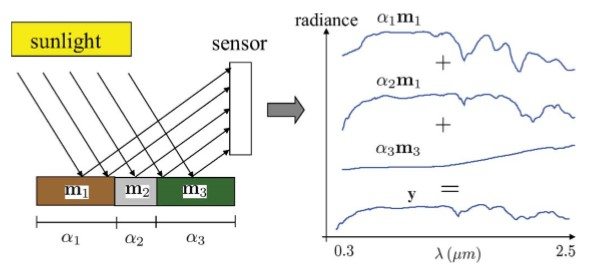
\includegraphics[width=0.9\linewidth, height=5cm]{Picture2} 
 		%\caption{Caption1}
 		\label{fig:subim1}
 		\centering
 		 	\caption{Linear Unmxing, he measured radiance at a pixel is a weighted average of the radiances of the materials present at the pixel}
 	\end{figure}
 
Conversely, nonlinear mixing is usually due to physical interactions between the light scattered by multiple materials in the scene. These interactions can be at a classical,or multilayered, level or at a microscopic, or intimate, level. Mixing at the classical level occurs when light is scattered from one or more objects, is reflected off additional objects, and eventually is measured by hyperspectral image.\\
 	
Most of this overview is devoted to the linear mixing model.
The reason is that, despite its simplicity, it is an acceptable
approximation of the light scattering mechanisms in many real
scenarios.


\begin{figure}{}
	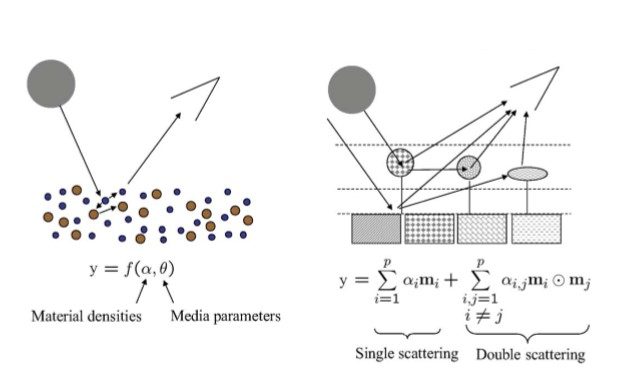
\includegraphics[width=0.7\linewidth, height=7cm]{Picture3} 
	%\caption{Caption1}
	\label{fig:subim1}
	\centering
	\caption{Non-Linear Unmxing}
\end{figure}

 
%\begin{eqnarray*}
%  \dot{x}&=&JH' (t,x)\\
% x(0) &=& x(T)
%\end{eqnarray*}
%with $H(t,\cdot)$ a convex function of $x$, going to $+\infty$ when
%$\left\|x\right\| \to \infty$.

\section{Dataset}
For the SNR-SD estimation, we have used the following datasets:
\begin{itemize}
	\item SudP5SNR40: simulated; mixing matrix sampled from a uniformly distributed random variable in the interval $[0,1]$
	\item SusgsP5SNR40: simulated; mixing matrix sampled from the United States Geological Survey (USGS) spectral library
	\item Rcuprite : real; subset of the well-known AVIRIS cuprite data cube 3 with size 250 lines by 191 columns by 188 bands (noisy bands were removed)
\end{itemize}
For the greedy sparse approximation:

 The experiments with the synthetic data are important because they provide quantitative evaluation of the approach, which is not possible with the real-world data. In all the experiments we used a fixed dictionary, which was created from the NASA Jet Propulsion Laboratorys Advanced Space-borne Thermal Emission and Reflectance Radiometer (ASTER) spectral library (http://speclib.jpl.nasa.gov). This library contains pure spectra of 2400 materials.\\
 
 To perform the experiments, we selected 425 of these spectra and resampled them in the wavelength range $0.4$ to $2.5 \mu m$, at a constant interval of $10nm$. The resampling is performed to match the sampling strategy of the NASAs Airborne Visible and Infrared Imaging Spectrometer (AVIRIS). We dropped 24 bands of the spectra in the dictionary because of zero or very low reflectance values. This made $D$ a $200 \times 425$ matrix. The spectra were selected such that $\mu = 0.9986$ for the dictionary. We kept $\mu < 1$ in order to ensure that the spectra in the dictionary are unique.\\
 
 The synthetic hyperspecral data is simulated the  with 500 mixed pixels, where each pixel was a linear combination of p randomly selected spectra from the dictionary. Following the experimental protocol, the fractional abundances of the endmembers in each pixel is drawn from a Dirichlet distribution. Therefore, the fractional abundances satisfy ASC(Abundance Sum-to-one Constraint). Gaussian white noise is then added to the data such that the pixels had $SNR = 50dB$. 
 
 
 
 MATLAB Code for creating synthetic image \\
 \hline
 \inputminted{octave}{createImage.m}
 \hline
 \vspace{0.5cm}
 Code for dirichlet sampling distribution:\\
 \hline
 \inputminted{octave}{dirichletSampling.m}
\hline





\section{Methodology}
%
\subsection{Linear Mixing Model}
If the multiple scattering among distinct endmembers is negligible and the surface is partitioned according to the fractional abundances, then the spectrum of each pixel is well approximated by a linear mixture of endmember spectra weighted by the corresponding fractional abundances. In this case, the spectral measurement at channel $i \in \{1,\allowbreak\dots,\allowbreak,B$ (B is the total number of channels) from a given pixel, denoted by, is given by the \emph{Linear Mixing Model} (LMM)

\begin{figure}{}
	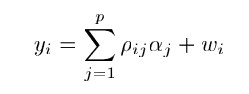
\includegraphics[width=0.35\linewidth, height=2cm]{Picture4} 
	%\caption{Caption1}
	\label{fig:subim1}
	\centering
\end{figure}

where $\rho_{ij} \geq 0$ denotes the spectral measurement of endmember $j \in \{1,\allowbreak\dots,\allowbreak,p$ at the $i^{th}$ spectral band,
 $\alpha_{j} \geq 0$ denotes the fractional abundance of endmember $j$, $w_{i}$ denotes an additive perturbation (e.g., noise and modeling errors), and $p$ denotes the number of endmembers. At a given pixel, the fractional abundance $\alpha_{j}$, as the name suggests, represents the fractional area occupied by the the endmember. Therefore, the fractional abundances are subject to the following constraints.
 \begin{equation}
 Non-Negativity \hspace{2cm} \alpha_{j} \geq 0
 \end{equation}
  \begin{equation}
Sum-to-One \hspace{2cm} \sum_{i}^{p} \alpha_{j} = 1
\end{equation}

\subsection{Characterization of the Spectral Unmixing Inverse Problem}
Given the data set containing $n$ $B-$dimensional spectral vectors, the linear HU problem is, with reference to the linear model, the estimation of the mixing
matrix $M$ and of the fractional abundances $\alpha_{i}$ vectors corresponding to pixels $i = 1.. .. n$
The Inverse Problem of finding the endmembers by a linear model is often a difficult inverse problem, because the spectral signatures tend to be strongly correlated, yielding badly-conditioned mixing matrices and, thus, HU estimates can be highly sensitive to noise. To characterize the linear HU inverse problem, we use the \emph{Signal-to-Noise-Ratio Spectral Distribution (SNR-SD)} 
 \begin{equation}
SNR-SD(i) = \frac{\lambda_{i,x}}{e_{i,x}^T R_{w} e_{i,x}}
\end{equation}
For us to obtain any valid and acceptable results, it is necessary that this ratio is $\gg 1 $, else it will lead to closely spaced endmembers. If there is too much noise in the spectral response, then the unmixing does not give any proper desired results. Therefore, we must apply various correction like topographic correction, atmospheric corrections, etc. before doing any further processing like unmixing or band reduction on the image. The value is plotted on a semi log scale.

 MATLAB Code for calculation of the SNR-SD noise estimates:\\
\hline
\inputminted{octave}{snr_sd.m}
\hline



\subsection{Greedy Sparse Approximation} 
A greedy algorithm is an algorithmic paradigm that follows the problem solving heuristic of making the locally optimal choice at each stage with the intent of finding a global optimum. In many problems, a greedy strategy does not usually produce an optimal solution, but nonetheless a greedy heuristic may yield locally optimal solutions that approximate a globally optimal solution in a reasonable amount of time.\\

Greedy algorithms approximate the signal $y$ by iteratively selecting the atoms of the dictionary. \emph{Dictionary} here refers to the spectral library, which is a collection of the spectral signatures of pure materials at a series of wavelengths. The word \emph{Atom} represents here a material chosen from the spectral library. These atoms are selected such that the signal is approximated in minimum number of iterations. This greedy heuristic finally results in a sparse solution. We can unify the greedy sparse approximation algorithms under a base-line algorithm, which can be stated as the following sequential steps: 
\begin{enumerate}
	\item Identification of the atom(s) of D, best correlated to the residual vector of the current approximation of $y$. For initialization, $y$ itself becomes the residual vector.
	\item Augmentation of a selected subspace with the identified atom(s). The selected subspace is empty in the first iteration.
	\item  Residual update, after approximating $y$ with
	the selected subspace. 
\end{enumerate}

The above steps are repeated until some stopping rule is satisfied by the algorithm. Recently proposed greedy algorithms vary in different steps of the base-line algorithms. \\

Hyperspectral data has its own characteristics, such  as, the cardinality of a mixed  pixel  in  an  image  is  usually  small (four  to  five)  but  unknown,  the  spectra  of  different  materials (i.e.  the  atoms  of  the  library)  are  highly  correlated  and  the fractional abundances are non-negative quantities. The greedy sparse approximation algorithms were not  originally  proposed  for  hyperspectral  unmixng,  therefore they  do  not  explicitly  take  care  of  the  above  mentioned characteristics of the hyperspectral data. In fact, to the best of our  knowledge,  no  pixel-based  greedy  sparse  approximation algorithm has ever been proposed specifically for the problem of sparse unmixing of hyperspectral data.\\

The \emph{Sparse  Unmixing  via  Greedy  Pursuit} (SUnGP) is a  pixel-based  greedy  algorithm  that  has  been  designed particularly for the problem of hyperspectral unmixing. Each  iteration  of  the  algorithm  comprises  the  three  steps  of  the  base-line  algorithm.  In  the identification step,  SUnGP  first  computes the  correlations  between  the  atoms  of  the  dictionary  and  the residual  vector  of  the  current  approximation  of $y$,  where $y$ itself is considered as the residual vector at initialization.\\

Then, SUnGP identifies the atoms of the dictionary corresponding to the $L$(an algorithm parameter) largest values of the computed correlations. These atoms are used for temporarily augmenting the selected subspace. Using this subspace, a non-negative least squares  approximation  of  the  mixed  signal  is  computed  (line‘8’ in Algorithm 1). SUnGP then identifies the atom from the aforementioned $L$ atoms  that  has  the  maximum  contribution
in  this  approximation.  This  atom  is  used  for  permanently
augmenting the selected subspace (line ‘10’).\\

Notice that, SUnGP first identifies a subspace of $L$ atoms (which  are  highly  correlated)  and  later  prunes  it  keeping  in view  the  non-negativity  of  the  solution  space,  to  identify  the single best atom. Once the best atom is identified, it is added to the selected subspace, never to be dropped off in the future iterations. This strategy stems directly from the aforementioned
characteristics of the hyperspectral data. SUnGP follows OMP(Orthogonal matching
pursuit) in  the residual  update step  and  uses  a  disjunction  of  three
stopping  rules (line  ‘13’).  The  rules  (a)  and  (b)  are  self
explanatory.  The  rule  (c)  ensures  that  the  algorithm  stops  if
it  is  not  able  to  reduce  the $l_{2}$ norm  of  the  residual  vector  at
least by a fraction $\beta$ in its last iteration. The rules (b) and (c)
allow  SUnGP  to  operate  without  prior  information  about  the
cardinality of the mixed pixel.\\

In   the   sparse   approximation   literature,   the   correlation
among  the  atoms  of  the  dictionary  is  usually  quantified  by
the mutual coherence $\mu \in [0,1]$, of the dictionary.
Researchers at the German Aerospace Center have shown that  for  a  dictionary  of  spectra  sampled  at  a  constant  wavelength interval, $\mu$ can be reduced by taking the derivatives of the spectra. The derivative of a spectra $d \in R^{m}$ is defined as
\begin{equation}
    \Delta(d) = \frac{d(b_{i}) - d(b_{j})}{b_{i} - b_{j}} \hspace{1cm} \forall \hspace{1cm} i \in {m...c}
\end{equation}

where $b_{z}$ is the wavelength at the $z^{th}$ band, $ d(b_{z})$ is the reflectance value at that wavelength and $j=i+c$, where $c$ is being positive integers.\\

\begin{figure}[h]
	\centering
	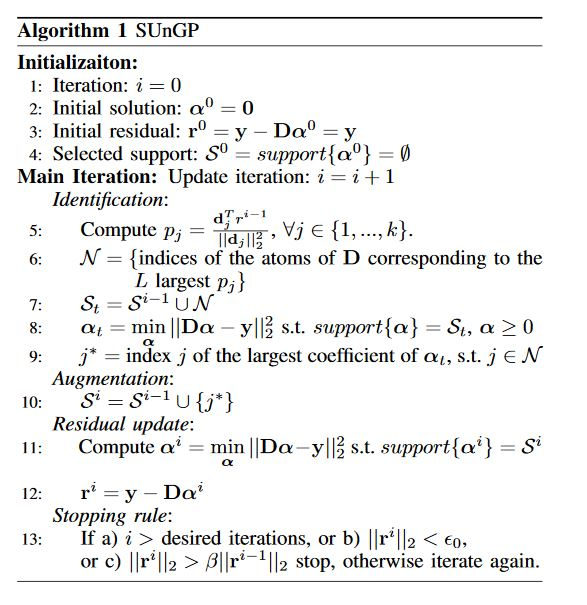
\includegraphics[width=0.8\linewidth, height=13cm]{Picture8} 
	\caption{Designed greedy sparse algorithm }
	\label{fig:algo}
\end{figure}

\hline
\inputminted{octave}{SUnGP.m}
\hline
\vspace{1cm}
Keeping in view its coherence reduction ability, we benefit
from  the  derivative  operation  in  hyperspectral  unmixing  with
the greedy algorithms. The following strategy is used for processing the hyperspectral data for the greedy sparse approximation algorithms:

\begin{enumerate}
    \item Create the dictionary $D_{\Delta}$ and the pixel $y_\Delta$ by taking
the  derivative  of  each  spectra  in $D$ and  the  pixel $y$, respectively:\\
\hline
\inputminted{octave}{SpecDerivative.m}
\hline
\vspace{5mm}
    \item Compute $\alpha$ with  the  greedy  sparse  approximation algorithm using $D_{\Delta}$ and $y_\Delta$.
    \item Estimate  the  fractional  abundance  vector $\Bar{\alpha}$,  by  the non-negative least squares approximation of $y$ using the atoms of corresponding to the support of $\aplha$.\\
    \hline
    \inputminted{octave}{Sugnp_code.m}
    \hline
\end{enumerate}
 
The  unmixing  performed  on  the  differentiated  data  in
step (2) is used to identify the correct support of the solution.
Once the support is found, it is used for the actual estimation of
the fractional abundances using the original data in the step (3).
In the above strategy, we use the dictionaries after normalizing
their atoms in $l_{1}$ norm.\\

By doing so, the estimated fractional
abundances automatically satisfy ASC. It is worth mentioning
here that the derivative operation helps in coherence reduction,
however the correlation among the spectra of the differentiated
data still remains high enough to cause problems for the greedy
sparse  approximation  algorithms.  Therefore,  the  algorithms
need to show robustness against the correlation of the spectra
for effective hyperspectral unmixing.

The error associated and the fidelity is also calculated.

\section{Results and Discussion}
\begin{figure}{}
	\centering
	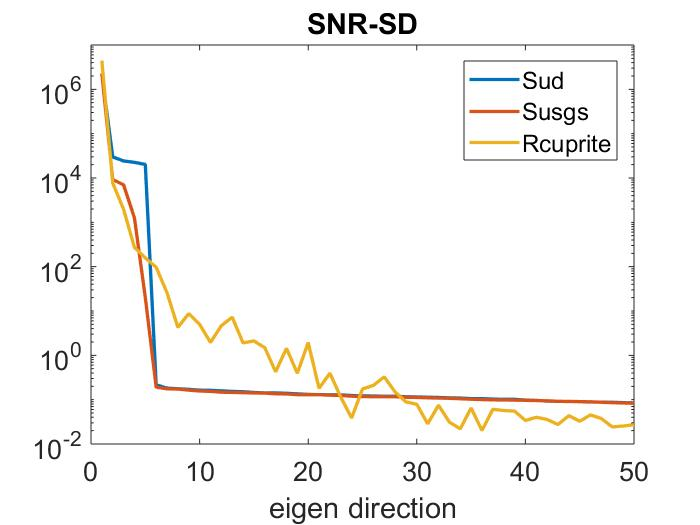
\includegraphics[width=0.8\linewidth, height=7cm]{Picture5} 
	\caption{ Signal-to-noise-ratio spectral distribution (SNR-SD)  }
	\label{fig:res1}
\end{figure}
We first analyse the linear mixing model overviewed above. We review the dataset by performing characterisation of the spectral unmixing inverse problem using the SIgnal-to-Noise Spectral Distribution(SNR-SD). We do so not only on the real CUPRITE dataset of AVIRIS-NG, but we also apply it on simulated or artificially made images as listed below.\\


Fig. \ref{fig:res1} plots , in the interval , for the following data sets:
\begin{itemize}
	\item SudP5SNR40: simulated; mixing matrix sampled from a uniformly distributed random variable in the interval $[0,1]$
	\item SusgsP5SNR40: simulated; mixing matrix sampled from the United States Geological Survey (USGS) spectral library
	\item Rcuprite : real; subset of the well-known AVIRIS cuprite data cube 3 with size 250 lines by 191 columns by 188 bands (noisy bands were removed)
\end{itemize} 

From the result, we can observe that the ratio has fallen to a value less than 1 quite fast.
The signal and noise correlation matrices were obtained with the
algorithms and code distributed with \emph{HySime}. From those plots, we read that, for SudP5SNR40 data set $SNR-SD(i) \gg 1$  for $i\leq5$, thus displaying a high signal subspace.\\

For SusgsP5SNR40, the singular values of the mixing matrix decay faster due to the high correlation of the USGS spectra lsignatures. Never the less it is very much similar to that of SudP5SNR40 dataset.\\

The Rcuprite data set yields the more difficult inverse problem
because has “close to convex shape” slowly approaching the value 1. This is a clear indication of a badly-conditioned inverse problem.\\


\begin{figure}{}
	\centering
	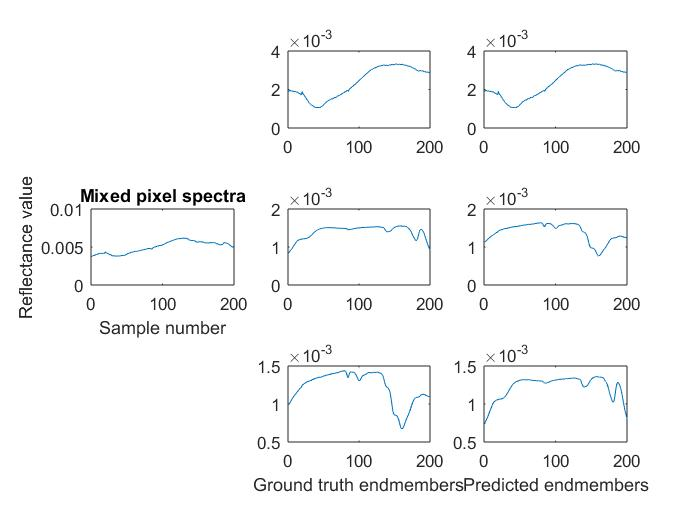
\includegraphics[width=0.8\linewidth, height=7cm]{Picture7} 
	\caption{ Greedy Algoithm results on artificial image }
	\label{fig:res2}
\end{figure}

The  values  in  these  results,  and  the  results  to  follow,  are
the  mean  values  of  the  metrics,  computed  over  the  whole
synthetic  data.  The  results  show  that  SUnGP  performs  better
than  the  existing  greedy  sparse  approximation  algorithms.
For  SUnGP  we  used $L=  50$,  which  was  optimized  on  a
separate  training  data  set.  Different  parameters  of  the  other
algorithms were also optimized on the same training data set.
We have given the correct values. The  algorithms  corresponding  to  these \ref{fig:res2} assume  a  priori  knowledge  of $p$
.  Therefore,  they  are  not  of practical  use  in  hyperspectral  unmixing.  However, it is used in the analysis for a comprehensive comparison
of  SUnGP’s  performance  with  the  state  of  the  art  greedy
algorithms.\\

In the figure \ref{fig:res2}, we can see the mixed pixel spectra which represents a synthetic image on which unmixing has to be performed. This image is made from a combination of 3 randomly selected endmembers from the spectral library. The groundtruth endmembers are shown in the middle column of the image. After running the greedy algorithm code, we get the predicted endmembers. \\

We can see that the predicted endmembers are not exactly the same as the groundtruth endmembers. This is because the greedy algorithm is an approimation method to to get the most optimised result. It has been modified to suit the problem statement of Hyperspectral Unmixing.  However, there may be times when this algorithm may not yield desired results.\\

However, we can notice that there is not much difference between the predicted and groundtruth enmembers for this image which is a clear indication of a quite fair accuracy. 





\subsection{Conclusion}


Hyperspectral unmixing is a challenging practical problem for unsupervised learning.The algorithm proposed by \emph{Naveed Akhtar, Faisal Shafait and Ajmal Mian} presents a pixel based greedy sparse approximation algorithm, called SUnGP, for hyperspectral unmixing. The proposed algorithm identifies different spectra in a mixed hyperspectral pixel by iteratively selecting a subspace of spectra from a fixed dictionary and pruning it. The algorithm has been shown to
outperform the existing state of the art greedy sparse approximation algorithms. Also, we reviewed ways to identify if the problem of linear Mixing Model (LMM) can suit a given dataset with respect to noise characteristics by analysing the Signal-to-Noise Ratio spectral distribution. 
The scope of this field of research is vast and unlimited. However, we limit the scope of this project to reviewing some simple proposed techniques for unmixing hyperspectral images.

\subsection{Acknowledgement}
I would like to acknowledge Ms. Amba Shetty for guiding me throughout the course of the project. Also, I would like to thank her for being a contant source of motivation for me to continue with this topic, which was a challenging and hard task.
I would also like to thank our faculty advisor, Ms. B R Jayalekshmi, for being supportive in proceeding with the course. 





\section{References}
\emph{
\begin{enumerate}
    \item Akhtar, Naveed, Faisal Shafait, and Ajmal Mian. "SUnGP: A greedy sparse approximation algorithm for hyperspectral unmixing." 2014 22nd International Conference on Pattern Recognition (ICPR). IEEE, 2014.
    \item Bioucas-Dias, José M., et al. "Hyperspectral unmixing overview: Geometrical, statistical, and sparse regression-based approaches." IEEE journal of selected topics in applied earth observations and remote sensing 5.2 (2012): 354-379.
    \item Parra, Lucas C., Clay Spence, Paul Sajda, Andreas Ziehe, and Klaus-Robert Müller. "Unmixing hyperspectral data." In Advances in neural information processing systems, pp. 942-948. 2000.
    \item Drumetz, Lucas, et al. "Blind hyperspectral unmixing using an extended linear mixing model to address spectral variability." IEEE Transactions on Image Processing 25.8 (2016): 3890-3905.
    \item Code Source for the greedy sparse approximation algorithm:  (http://staffhome.ecm.uwa.ed\\u.au/~00053650/code.html)
    \item Sources: http://openremotesensing.net/knowledgebase/code-and-demo-for-hyperspectral-u\\nmixing-2
    \item Sources: http://openremotesensing.net/?s=Hyperspectral+Unmixing+Overview$\%$3A+Geome\\trical$\%$2C+Statistical$\%$2C+and+Sparse+Regression-Based+Approaches&post$_$type=
\end{enumerate}
}
%
% ---- Bibliography ----
%\bibliographystyle{apalike}
%\bibliography{my_library}

%deeparamesh88@yahoo.com
%title-application of greedy algorithhm for unmixing of hyperspectral data.
%conclsuion- how efficient algorithm is for the present dataset
\end{document}
